\chapter{GoLightly} \label{ch:golightly}

GoLightly is the GPU-based FDTD simulator application that is the focus and product of this thesis. Written using a combination of C++, CUDA and OpenGL, it provides a lightweight yet complete FDTD solution.

\section{Goals}

GoLightly is intended to address deficiencies common to CPU-based solutions. In particular, it is designed to be fast, friendly and portable.


\begin{itemize}
	\item Fast. An iterative design process requires rapid feedback from the simulator. Long simulation times necessitated by existing solutions inhibit this process.
	\item Friendly. Definition of models and other simulation parameters should not require expertise in software development or quasi-proprietary scripting languages. 
	\item Portable. Ideally, the simulator should run on a high-end consumer grade laptop and support the most common desktop operating systems (Microsoft Windows and Apple OS X).  
\end{itemize}

To meet those goals, GoLightly takes advantage of the programmable GPU available in common desktop and laptop computers, resulting in a dramatic speedup. Rather than relying on a proprietary model definition language or obscure, limited scripting system, we use industry-standard image and geometry file formats so that models may be defined using robust, familiar, readily-available tools. 

\section{Architecture}

GoLightly comprises three primary application blocks:

\begin{itemize}
	\item Model Processor \ref{sec:modelProcessor}
	\item Simulator \ref{sec:simulator}
	\item Visualizer \ref{sec:visualizer}
\end{itemize}

\section{Model Processor}\label{sec:modelProcessor}

The model processor (MP) is responsible for initialization of the simulator. When launching the simulator, a domain size and image file containing a coded image of the desired dielectric as well as $\epsilon_{max}$ are specified.

\begin{table}[h!]
	\centering
	\caption{Model processor inputs}
	\label{tab:modelProcessorInputs}
	\begin{tabular}{l | l | l | l}
		Symbol	& Data Type & Meaning & Typical value				\\
		\hline														
		Width	& int 		& Domain size in X & 1024				\\
		Height	& int 		& Domain size in Y & 1024				\\
		Media	& float 	& $\epsilon_{max}$ & 9						\\
		Model	& string	& Model definition stored as a bitmap & filename \\
		$\epsilon_{max}$ & float & Maximum $\epsilon$ value for this model
	\end{tabular}
\end{table}

The MP allocates arrays to hold the dielectric properties for each Yee cell. These arrays are of the same dimensions as the domain, which may be different than the dimensions of the model to accomodate boundary cells.

Once the model image is loaded, the MP iterates through each pixel in the image. (See \autoref{listing:modelFromImage}), and parses each pixel to populate data structures describing the dielectric contents of the simulation as well as source and monitor locations and parameters.

For each element:

\begin{enumerate}
	\item Determine the normalized texel coordinate that corresponds to the current cell position	
	\item Read the red (R), green (G) and blue (B) color components from the image
	\item If $R > 128$, this texel is part of a source. Add the cell to the list of sources
	\item If $G > 0$, this texel has non-unity dielectric. Set ${C_b}_{i,j} = \epsilon_{max} * \frac{G}{255.0}$
	\item If $B > 0$, this texel is part of a monitor. Add its position to the monitor definition with ID = $B$
\end{enumerate}

Source code for the image processor is shown in listing \autoref{listing:modelFromImage}.

\lstinputlisting[language=c++,caption=Generating a model from an image,label={listing:modelFromImage}]{model-from-image.cpp}

Once the dielectric, sources and monitors are derived from the model image, the model processor transfers control to the simulator.

\section{Simulator}\label{sec:simulator}

The simulator block implements the FDTD algorithm. Given the dielectric, source and monitor configurations from the model processor, the simulator initializes the GPU, transfers required data from host memory to the GPU, and begins the simulation loop.

In addition to the dielectric and field arrays, the simulator generates a  descriptor (\ref{listing:fieldDescriptor}) for each field that will be updated. This structure is used by the kernels to assist in handling boundary conditions (PML) and other housekeeping duties. A similar, more compact  descriptor (\ref{listing:deviceFieldDescriptor}) is generated from the host descriptor and passed to the kernels.

\lstinputlisting[language=c++,caption=Host Field Descriptor structure,label={listing:fieldDescriptor}]{fieldDescriptor.cpp}

\lstinputlisting[label={listing:deviceFieldDescriptor},language=c++,caption=Device Field Descriptor]{deviceFieldDescriptor.cpp}

For each loop iteration, the simulator launches a CUDA kernel to update all $E$ fields. Once the $E$ update is complete, the simulator launches kernels to update all $H$ fields.

The three kernels required for a $TM_Z$ simulation are detailed below:

\lstinputlisting[label={listing:updateEzCpp},language=c++,caption={CUDA kernel for updating $E_Z$}]{cu_update_ez.cpp}

The majority of each kernel's source performs setup and bounds checking tasks. In each kernel, the FDTD equation implementation can be isolated to one or two lines of code.

For example, the line (from the $E_Z$ update kernel),

\begin{lstlisting}
	Ez->Data[center] = CA * Ez->Data[center] + cb * (dhy - dhx) + cb * (ezxPsi - ezyPsi);
\end{lstlisting}

corresponds to the FDTD $E_Z$ equation. (See \autoref{eq:ezupdate})

\lstinputlisting[language=c++,caption=CUDA kernel for updating $H_X$]{cu_update_hx.cpp}\label{listing:updateHxCpp}

\lstinputlisting[language=c++,caption=CUDA kernel for updating $H_Y$]{cu_update_hy.cpp}\label{listing:updateHyCpp}

Note that all $E$ updates occur simultaneously, as do all H fields. However, given the dependence between the $E$ and $H$ fields, the $E$ field update kernels must complete before the $H$ fields are updated.

The simulator repeats this operation until the application is closed, or the desired number of frames are completed. 

Finally, the completed field arrays are copied to the host from the GPU, and saved to disk in bitmap and CSV format for later analysis. 

\section{Visualizer}\label{sec:visualizer}

If enabled \footnote{The visualizer requires some GPU overhead. As such, its use may affect simulator performance.}, the visualizer application block provides interactive display of the simulation. 

When running a simulation, the user may optionally specify a visualizer update frequency, indicating the number of simulation frames that should complete between visualizer updates. This aids in reducing the visualizer's performance impact.

A window and OpenGL context are created using GLFW and the glLoadGen OpenGL extension loader. An OpenGL pixel buffer object (PBO) is allocated to contain a copy\footnote{The PBO may be of different dimensions than the simulation domain. Since the PBO is used only for visualization, it is not necessary for it to contain the full-resolution field.} of the field that the user wishes to observe\footnote{The visualizer provides the ability to dynamically select which field(s) should be displayed}. 

The visualizer also creates a screen-aligned quad on which the field texture will be rendered, and allocates a texture object which is then bound to the PBO\autoref{fig:visualizerUpdatePipeline}.

\begin{figure}[H]
	\centering
	\includegraphics[  width=0.5\textwidth,
	keepaspectratio]{visualizerPipeline.png}
	\caption{Visualizer Update Pipeline}
	\label{fig:visualizerUpdatePipeline}
\end{figure}



After the required number of frames have been completed, the visualizer launches a CUDA kernel which samples the selected field and populates the PBO. 

\lstinputlisting[language=c++,caption=CUDA kernel for updating visualizer pixel buffer object]{cuvisualizerupdate.cpp}

\lstinputlisting[language=c++,caption=GLSL Vertex Shader,label={lst:basicvert}]{basicvert.glsl}

\lstinputlisting[language=c++,caption=GLSL Fragment Shader, label={lst:basicfrag}]{basicfrag.glsl}

A completed PBO is bound to a uniform input for a shader (\autoref{lst:basicvert}, \autoref{lst:basicfrag}) listing which renders the texture to the visualizer window. This process runs continuously. However, the texture is only updated at the frequency requested by the user when the simulation was launched. 

\begin{figure}[H]
	\centering
	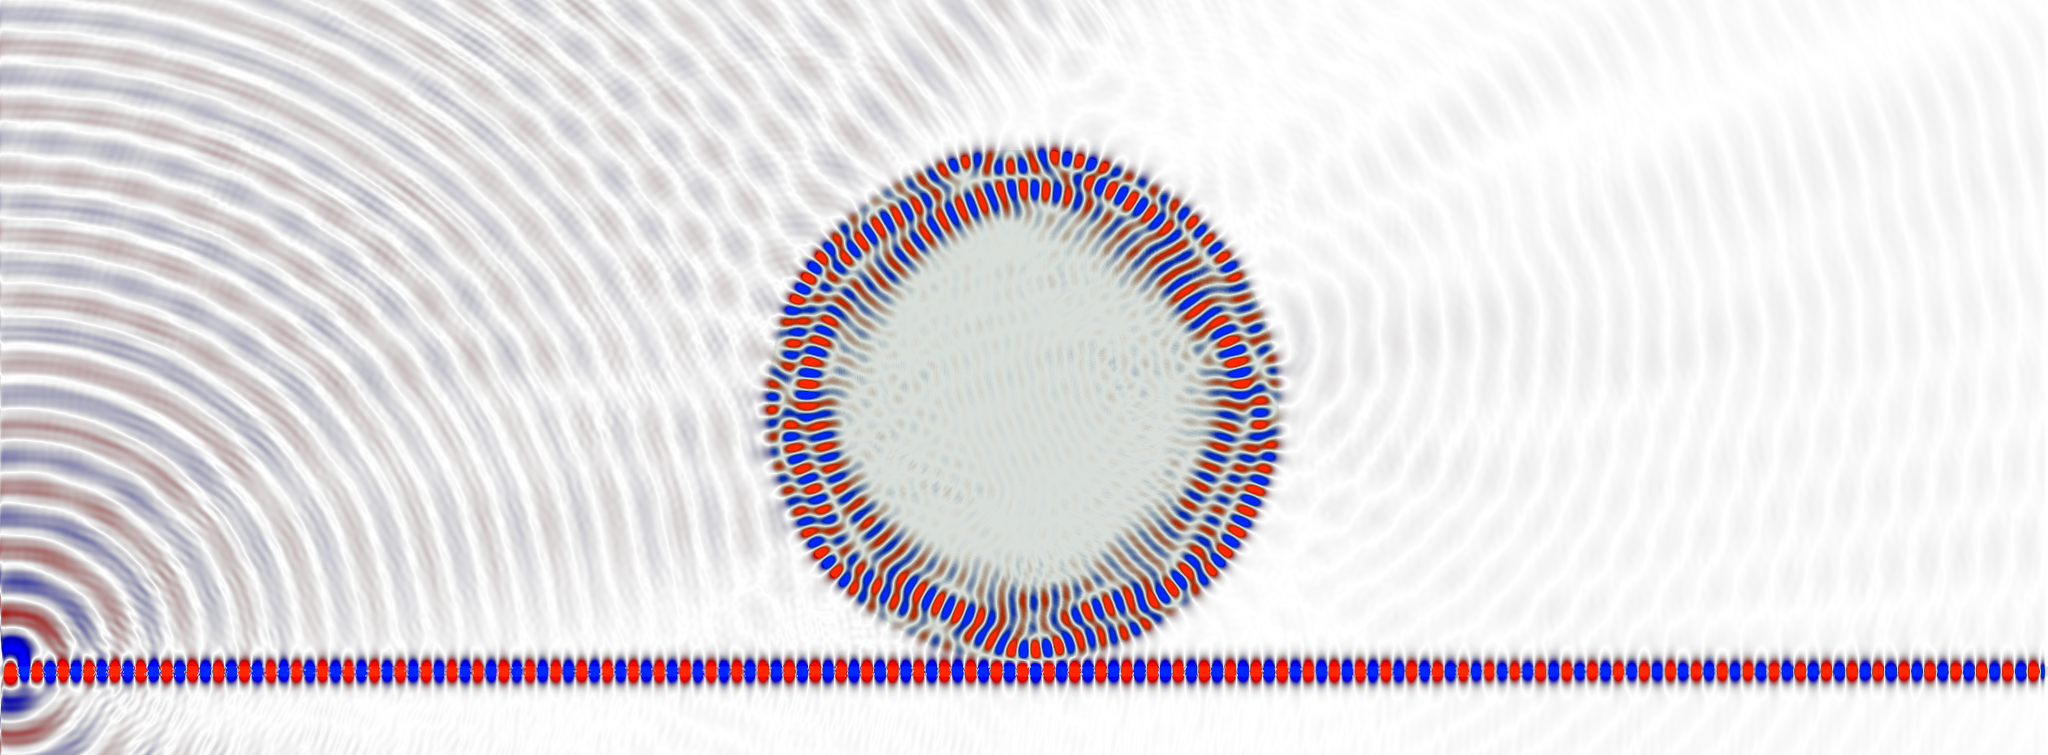
\includegraphics[  width=15cm,
	height=6cm,
	keepaspectratio]{visualizer-wgm.png}
	\caption{2D Whispering Gallery Mode Sensor}
	\label{fig:wgm}
\end{figure}

\clearpage

\section{Modeling approach}

For simplicity, models are defined in any of a number of standard 32-bit color image formats. In a 32-bit per pixel image, each color has 8-bit red, green, blue and alpha values. As mentioned in the model processor (\autoref{sec:modelProcessor}) section, each component is used to indicate some data about a given point in the simulation domain:

\begin{table}[h!]
	\centering
	\caption{Color component usage}
	\label{tab:modelColorComponentUsage}
	\begin{tabular}{l | l | l}
		Component	& Meaning & Interpretation\\
		\hline															 \\
		Red		& Source 				& normalized wavelength of the source \\
		Green	& Dielectric			& $\epsilon_r = green * \frac{\epsilon_{max}}{255.0}$ 	 \\		
		Blue	& Monitor				& ID of the monitor to which this texel belongs \\
		Alpha	& Reserved				& Reserved for future use. \\
	\end{tabular}
\end{table}

Whenever a non-zero blue (monitor) value is encountered, it is treated as an identifier ("ID") of a monitor. If the given ID has not yet been encountered, a new monitor is created. Any subsequent locations with the same ID are added to the corresponding monitor. This allows monitors to be of any shape or size.
 
Using a tool such as Adobe Photoshop or Microsoft Paint, the user can specify all required simulation input - sources, monitors and dielectric - in an intuitive fashion. Alternatively, these bitmaps could be generated by a custom tool which would voxelize a CAD model, assigning color components based on the model's metadata or object properties. 

A significant advantage of this approach over the CSG method used in Meep is that all constructs - sources, monitors and dielectric - can be of any shape that can be drawn in a bitmap. In theory, any voxel-based modeling tool could be used to build models in higher dimensions. 

\begin{figure}[H]
	\centering
	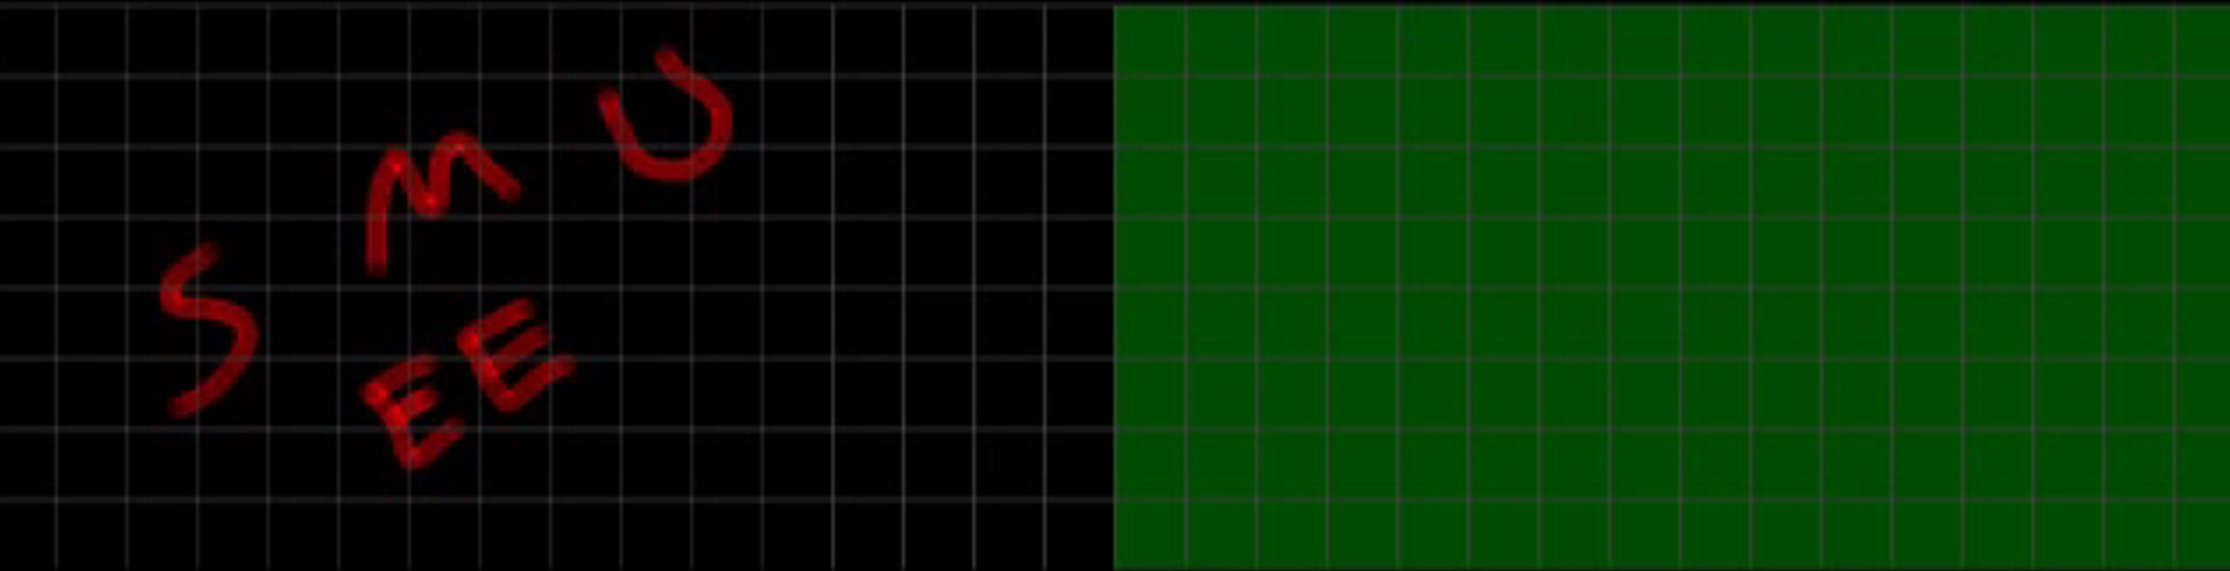
\includegraphics[  width=15cm,
	height=6cm,
	keepaspectratio]{arbitrary-source-shape.png}
	\caption{Arbitrarily-shaped source (Red pixels)}
	\label{fig:arbitrarySource}
\end{figure}

\begin{figure}[H]
	\centering
	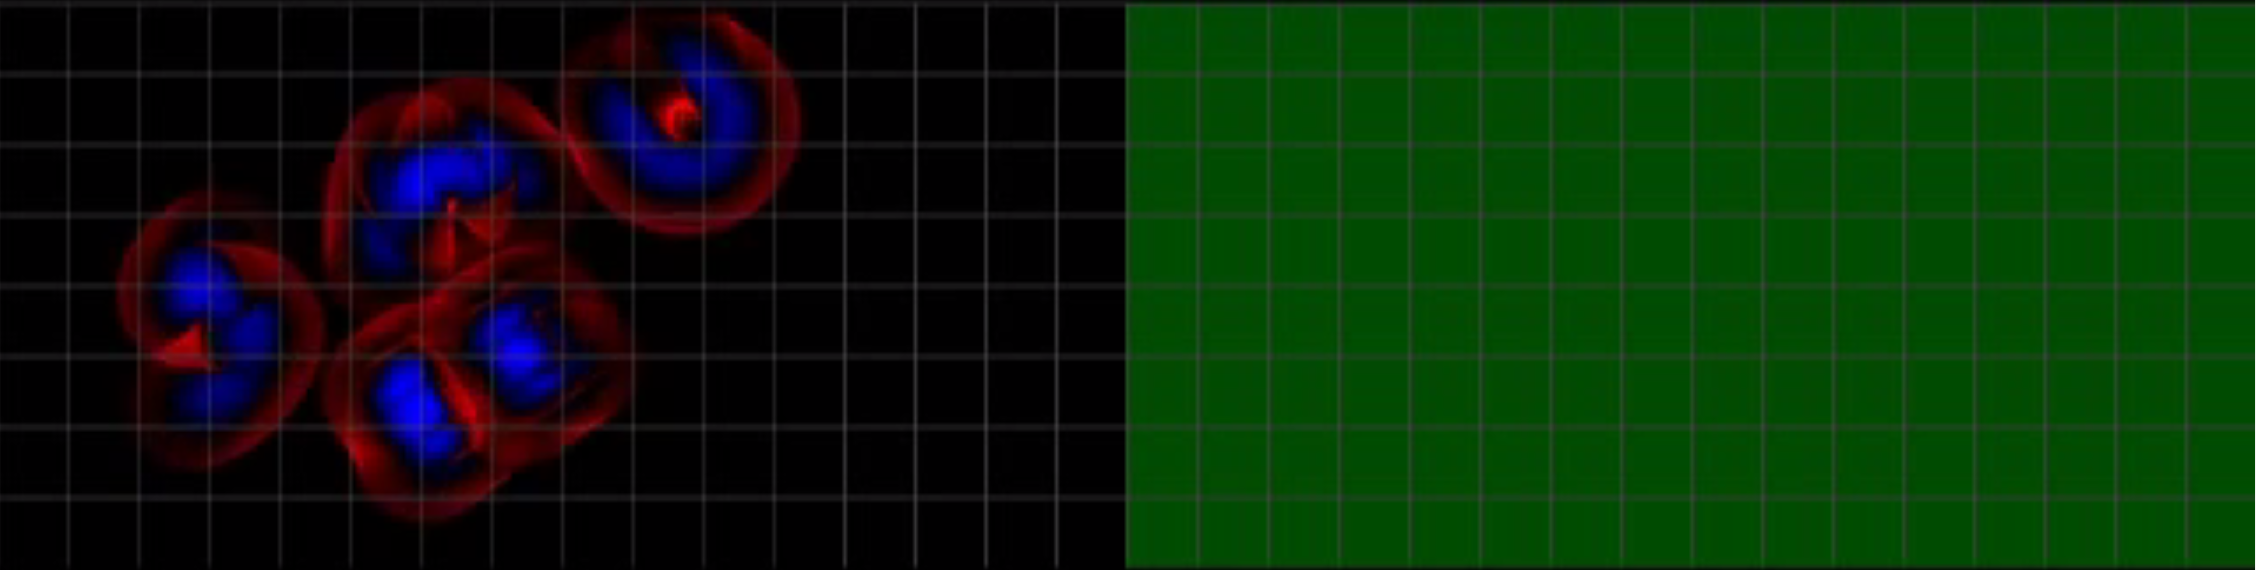
\includegraphics[  width=15cm,
	height=6cm,
	keepaspectratio]{arbitrary-source-shape2.png}
	\caption{Arbitrarily-shaped source after 20 frames}
	\label{fig:arbitrarySource2}
\end{figure}

\begin{figure}[H]
	\centering
	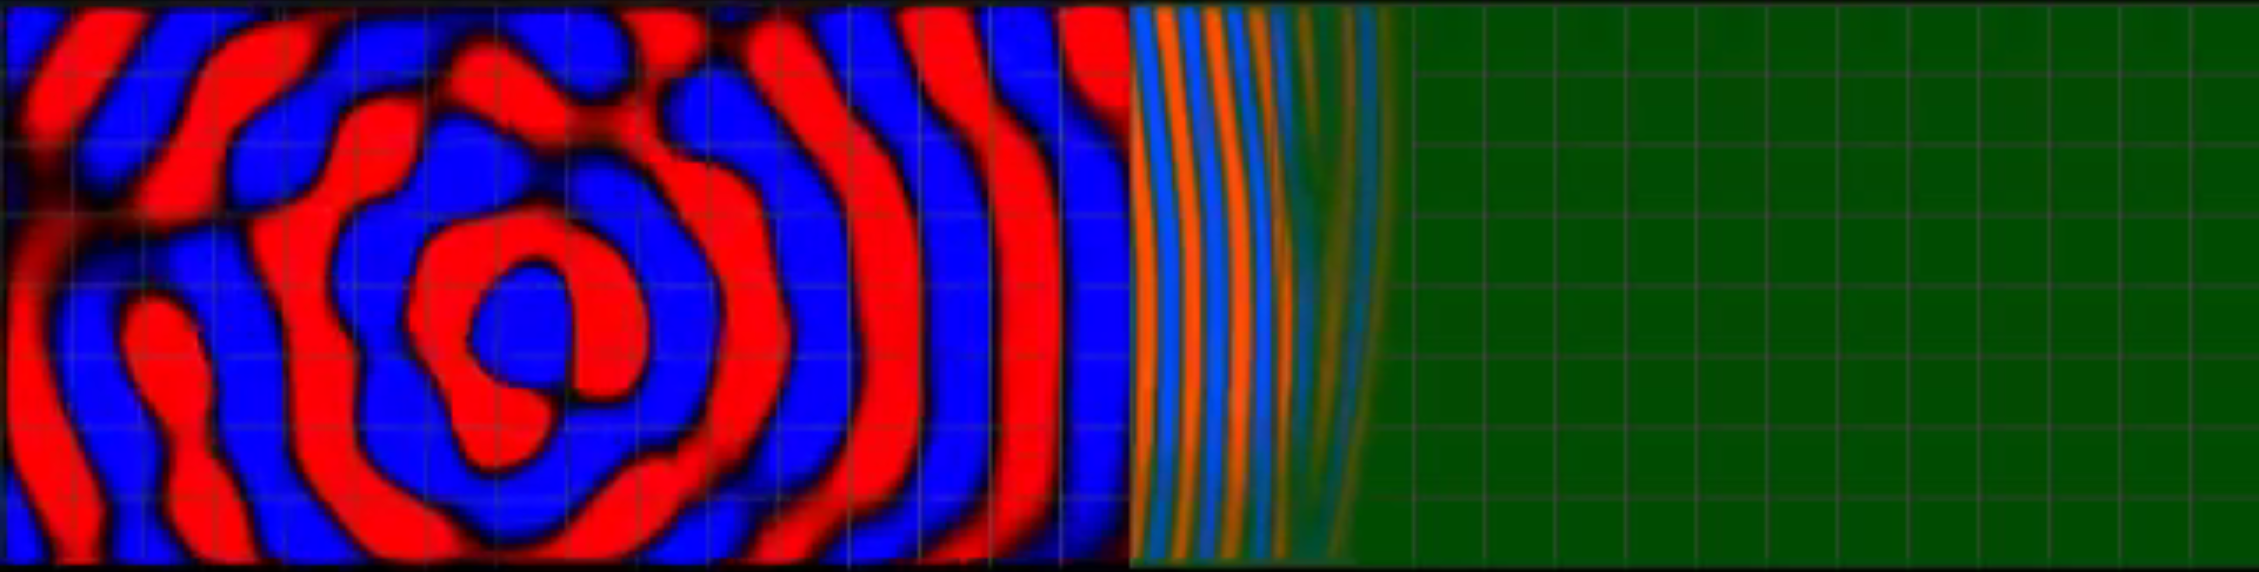
\includegraphics[  width=15cm,
	height=6cm,
	keepaspectratio]{arbitrary-source-shape3.png}
	\caption{Arbitrarily-shaped source after 100 frames}
	\label{fig:arbitrarySource3}
\end{figure}

\clearpage

\section{Testing and Validation Methodology}

In order to validate the GPU simulation results, a 2D $TM_Z$ simulation was executed.

\begin{figure}[H]
	\centering
	
\includegraphics[  width=15cm,
	height=6cm,
	keepaspectratio]{plane-wave-test-model.png}
	\caption{$TM_Z$ Test Model}
	\label{fig:plane-wave-test-model}
\end{figure}

As can be seen in \autoref{fig:plane-wave-test-model}, the simulation includes a plane wave source (red line), monitors for incident and transmitted waves (blue), and a dielectric slab with $\epsilon_R = 9$ (green). An additional monitor at the source location is not clearly visible due to it's relatively low ID (B = 5).

The simulation was first run with $\epsilon_R = 1$ to record the incident magnitude in absence of any reflective interfaces. The simulation was then run with $\epsilon_R = 9$ to record combined incidence and reflection, as well as transmittance within the dielectric.

In a post-processing step, the reflective magnitude was found by subtracting the incident wave magnitude obtained from the $\epsilon_R=1$ simulation from the combined incidence and reflection magnitudes obtained from the $\epsilon_R=9$ simulation.

Validation was performed by comparing the theoretical Fresnel coefficients for the test model with the time-averaged power (RMS) recorded during the simulation.

\subsection{Analytical Result}

In the test configuration, a normalized ($\lambda = 1$) $TM_Z$ plane wave is normally incident upon a dielectric interface with $\epsilon_R = 9$. 


\begin{figure}[H]
	\centering
	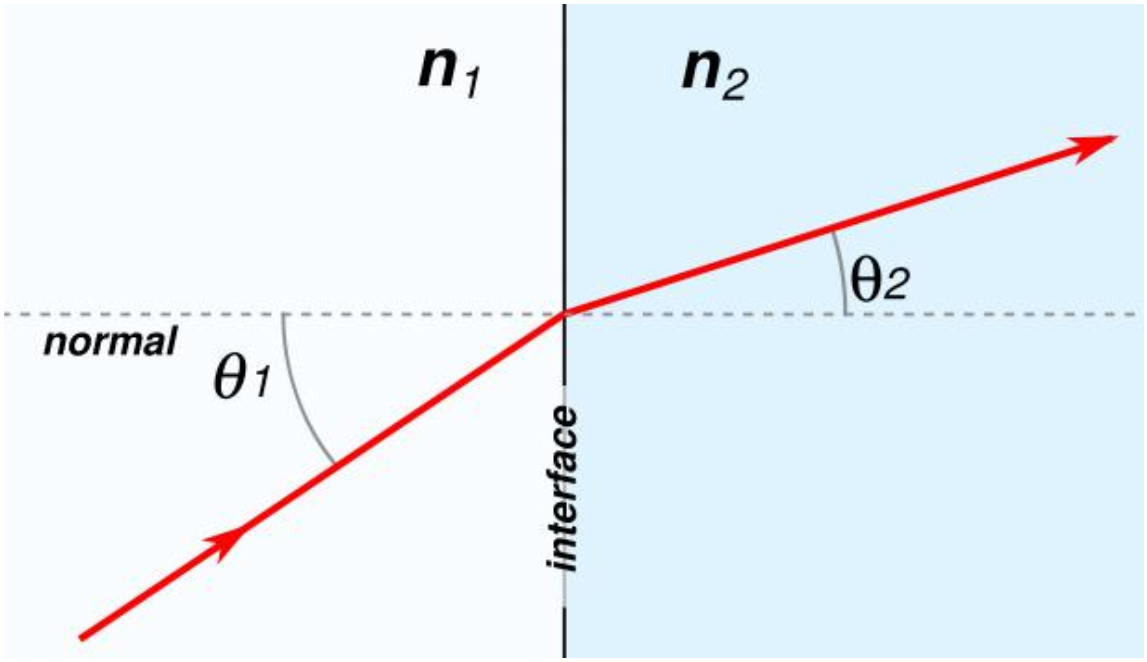
\includegraphics[  width=15cm,
	height=6cm,
	keepaspectratio]{snells-law.png}
	\caption{Snell's Law}
	\label{fig:snellslaw}
\end{figure}

Snell's Law states that the ratio of the refractive indices of the media at an interface, along with the angle of incidence, determine the angle of transmittance. (See \autoref{fig:snellslaw}) 

Mathematically, this relationship may be expressed as

\begin{equation}
n_1 \sin \theta_1 = n_2 \sin \theta_2
\end{equation}

In the test model, the index $n_2$ is calculated using the formula:

\begin{equation}
n = \sqrt{\epsilon_0 \epsilon_R \mu_0 \mu_R}
\end{equation}

In our simulator, $\epsilon_0$ and $\mu_0$ are normalized to 1. Similarly, in the non-magnetic media used in this case, 
\begin{equation}
\mu_R = 1
\end{equation}

Using our test value of $\epsilon_R = 9$ gives 

\begin{equation}
n_2 = \sqrt{9} = 3
\end{equation}

\clearpage

For a normally-incident plane wave, the incident and refraction angles are

\begin{equation}
\theta_I = 0
\end{equation}

and

\begin{equation}
\theta_T = 0
\end{equation}

Evaluating the Fresnel equations for the reflection and transmission of a $TM_Z$ wave,

\begin{equation}
r = \frac{n_2 \cos \theta_I - n_1 \cos \theta_T}{n_1 \cos \theta_T + n_2 \cos \theta_I}
\end{equation}
\begin{equation}
t = \frac{2 n_1 \cos \theta_I}{n_1 \cos \theta_T + n_2 \cos \theta_I}
\end{equation}

gives the coefficients:

\begin{equation}
r = \frac{3 * 1- 1 * 1}{1 * 1 + 3 * 1} = \frac{1}{2}
\end{equation}
\begin{equation}
t = \frac{2 * 1 * 1}{1 * 1 + 3 * 1} = \frac{1}{2}
\end{equation}

In this case, given a dielectric constant $\epsilon_R  = 9$, the reflection and transmission coefficients are equal.

\subsection{Numerical Result}

The observed steady-state output of the simulation for the baseline case ($\epsilon_R = 1$) is show in \autoref{fig:planewavefreespace}.

\begin{figure}[H]
	\centering
	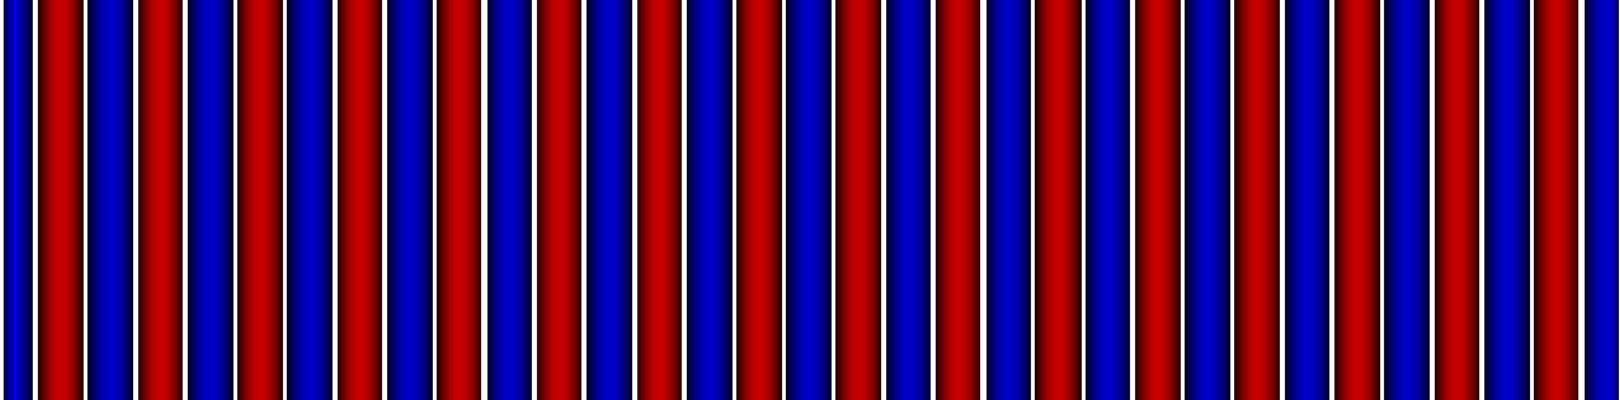
\includegraphics[  width=15cm,
	height=6cm,
	keepaspectratio]{plane-wave-free-space.png}
	\caption{Plane wave with $\epsilon_R = 1$}
	\label{fig:planewavefreespace}
\end{figure}

The time-averaged (RMS) numerical output for the incident and transmitted monitors is

\begin{figure}[H]
	\centering
	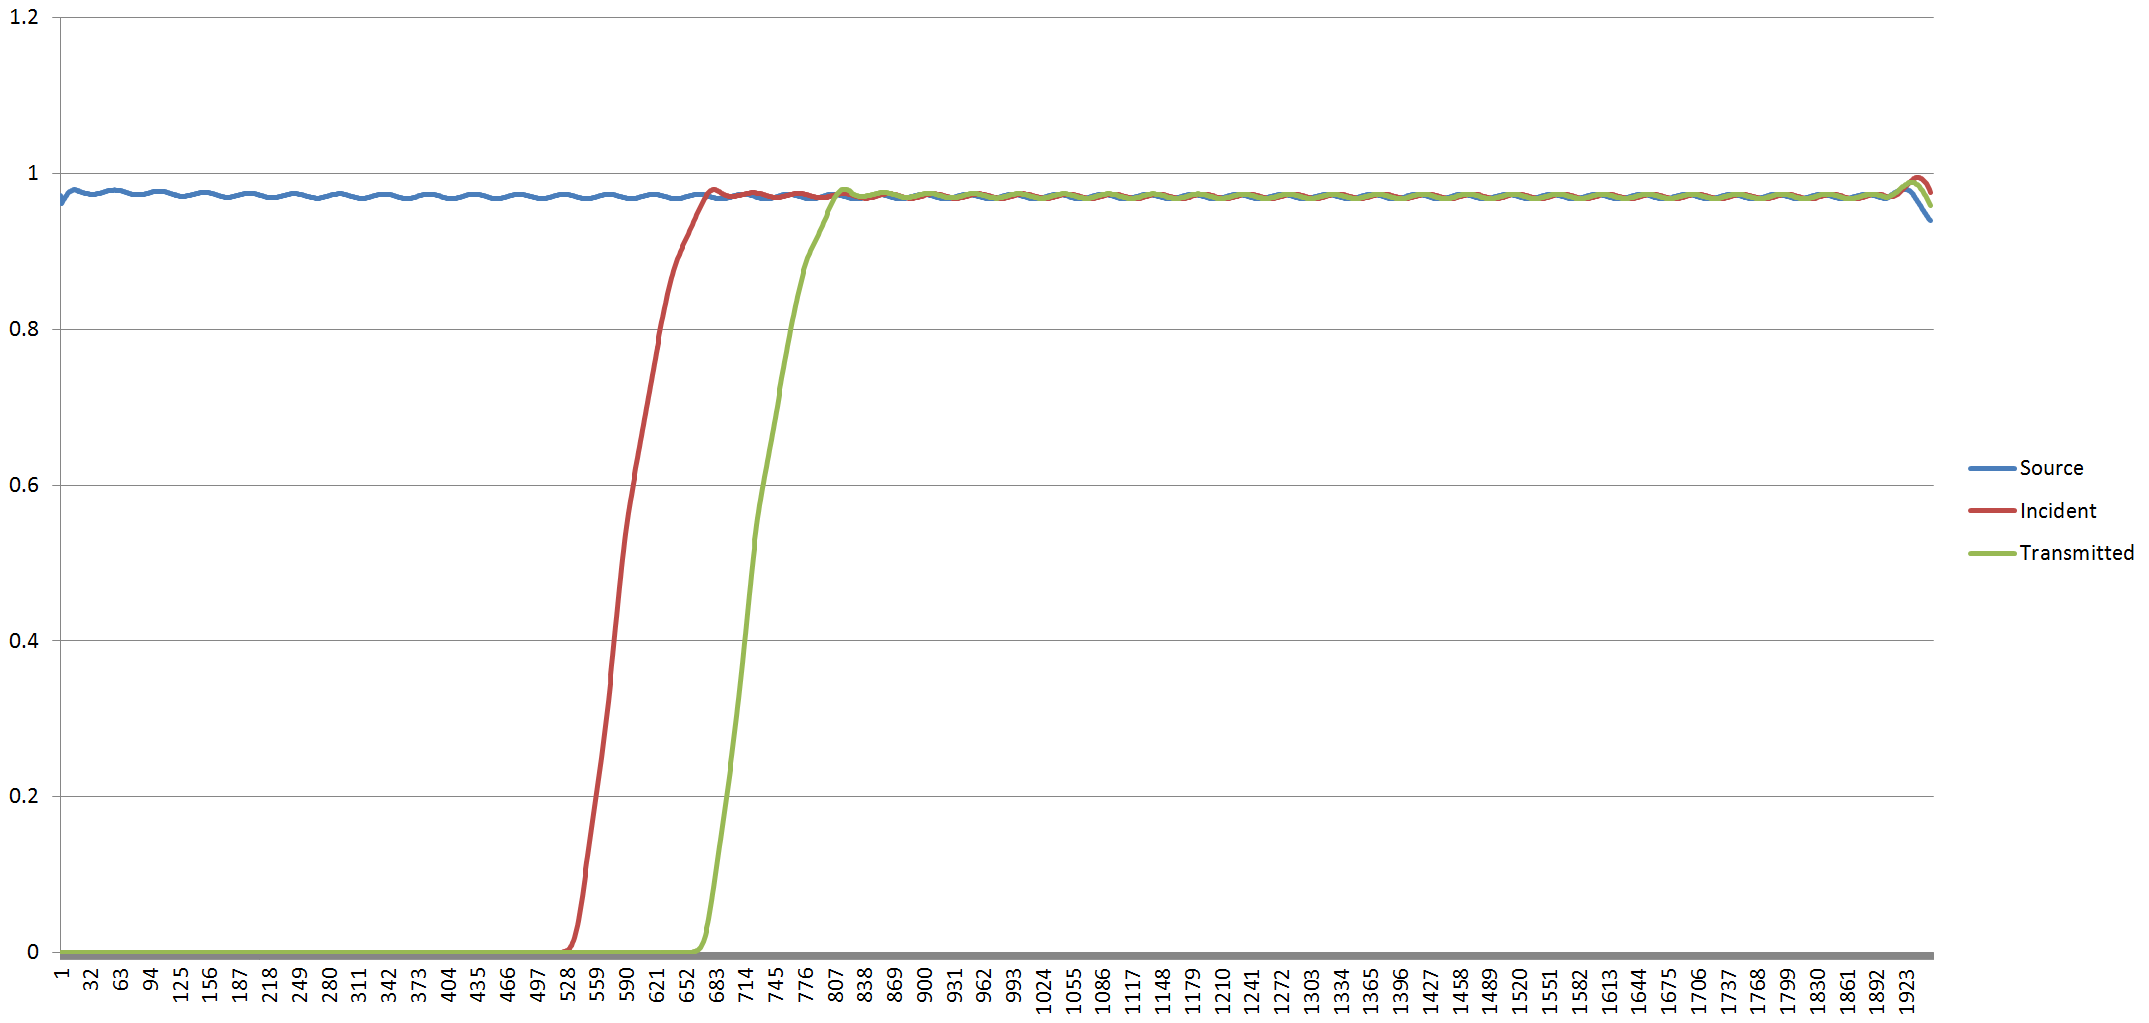
\includegraphics[width=\textwidth,
	keepaspectratio]{pw-time-averaged-output.png}
	\caption{Time-averaged (RMS) output in free space $\epsilon_R = 1$}
	\label{fig:planewaveRMSinFreeSpace}
\end{figure}

As expected, the incident and transmitted magnitudes equal the source magnitude, offset by the time it takes for the wave to propagate from the source to the monitors.

The observed output of the same simulation, executed with dielectric constant $\epsilon_R = 9$,

\begin{figure}[H]
	\centering
	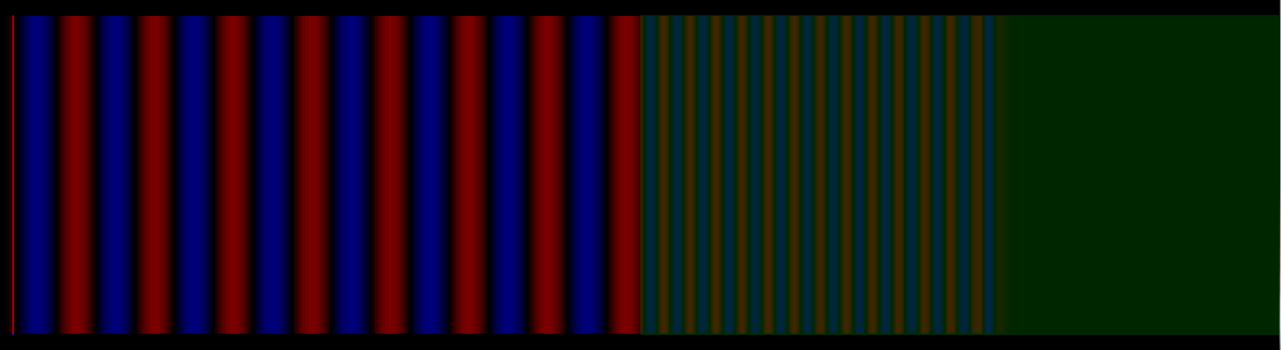
\includegraphics[width=\textwidth,
	keepaspectratio]{pw-epsilon-9.png}
	\caption{Steady state with $\epsilon_R = 9$}
	\label{fig:pwEpsilon9}
\end{figure}

Note the difference in $\lambda$ once the wave enters the dielectric (green area). This simulation produces the following raw output:

\begin{figure}[H]
	\centering
	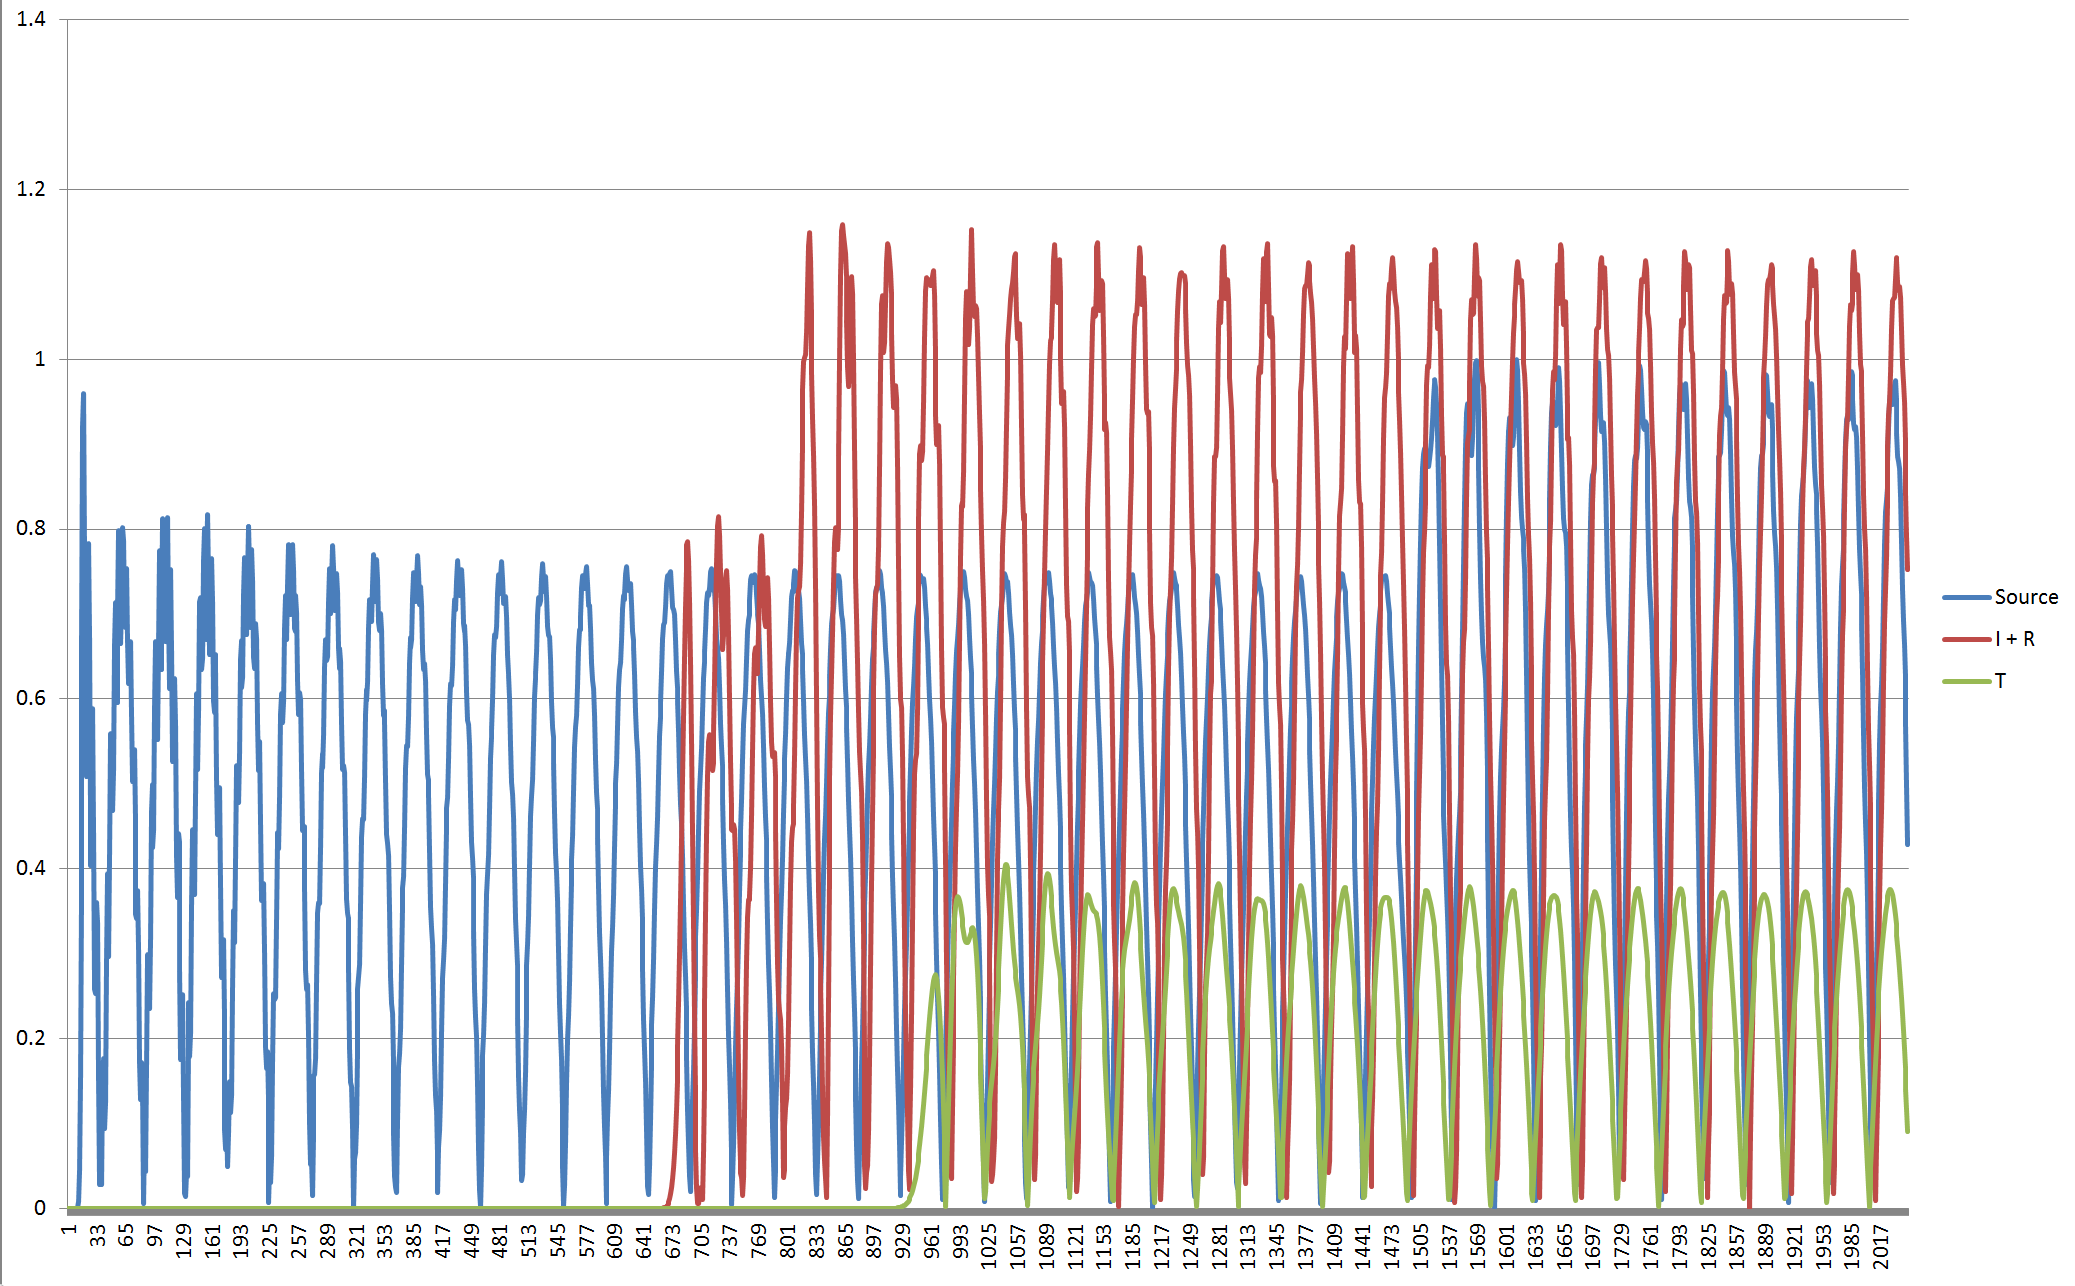
\includegraphics[width=\textwidth,
	keepaspectratio]{pw-epsilon-9-raw.png}
	\caption{Raw monitor output with $\epsilon_R = 9$}
	\label{fig:pwEpsilon9Raw}
\end{figure}

The time-averaged power for the monitors is shown in \autoref{fig:pwEpsilon9RMS}.

\begin{figure}[H]
	\centering
	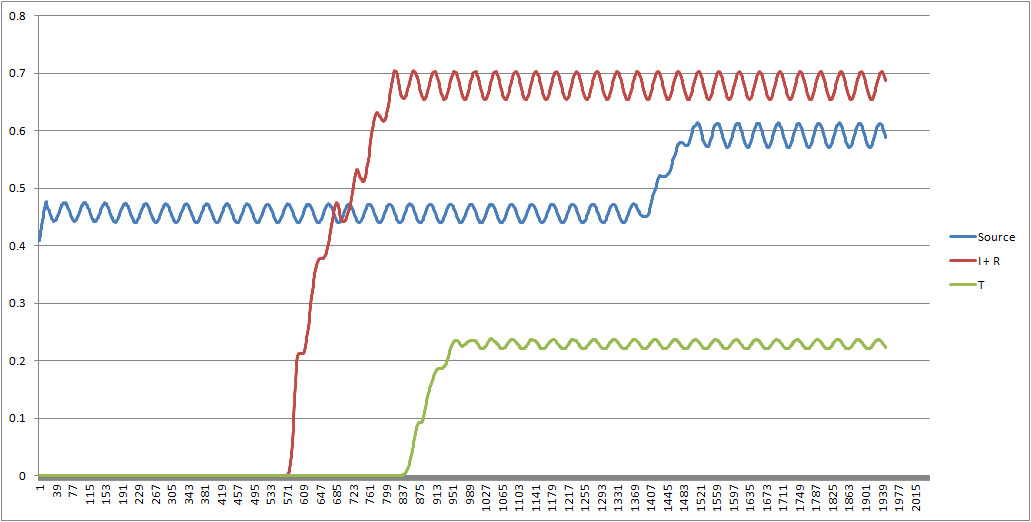
\includegraphics[width=\textwidth,
	keepaspectratio]{pw-epsilon-9-rms.png}
	\caption{RMS output with $\epsilon_R = 9$}
	\label{fig:pwEpsilon9RMS}
\end{figure}

Subtracting the incident magnitude from the simulation with $\epsilon_R = 1$ from the second simulation with $\epsilon_R = 9$ gives the following result (\autoref{fig:pwEpsilon9Normalized})

\begin{figure}[H]
	\centering
	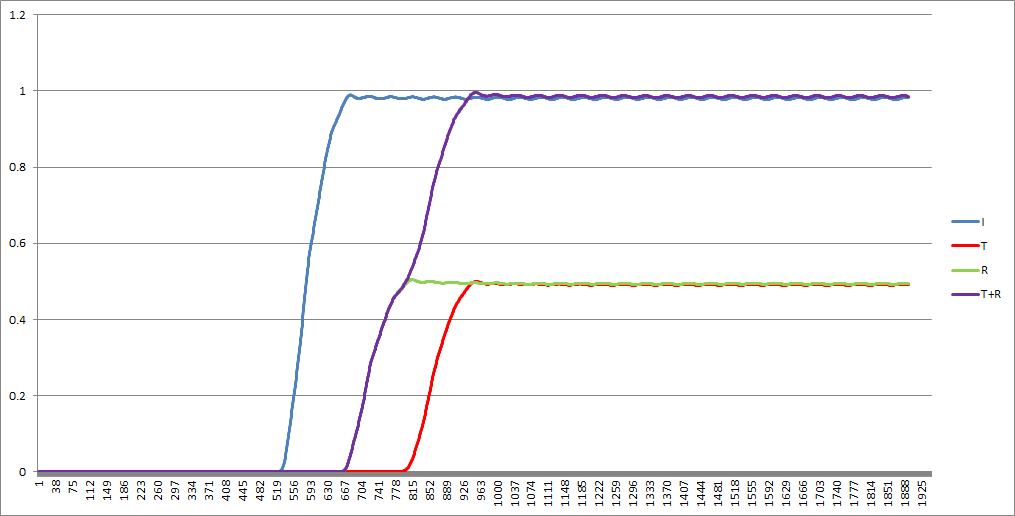
\includegraphics[width=\textwidth,
	keepaspectratio]{pw-epsilon-9-tir-power.png}
	\caption{Normalized output with $\epsilon_R = 9$}
	\label{fig:pwEpsilon9Normalized}
\end{figure}

In this case, the average of each of the relevant values are determined to be:

\begin{center}
$I_{avg} = 0.96214...$

$T_{avg} = 0.4882...$

$R_{avg} = 0.484...$
\end{center}

Conservation of energy requires that the sum of the transmitted (T) and reflected (R) magnitudes equals the incident magnitude (I).

\begin{equation}
I = T+R
\end{equation}

The computed error of the analytical result is

\begin{equation}
I_{error} = |\frac{I_{avg} - (T_{avg} + R_{avg})}{I_{avg}}|
\end{equation}

Gives

\begin{center}
	\begin{math}
	|\frac{0.9621-(0.4882 + 0.4843)}{0.9621}| = 1.011\%
	\end{math}
\end{center}

Comparing to the analytically-derived Fresnel coefficients,

\begin{equation}
T = \frac{T_{avg}}{I_{avg}} = \frac{0.4882219...}{0.962135...} = 0.507
\end{equation}
\begin{equation}
R = \frac{R_{avg}}{I_{avg}} = \frac{0.484332...}{0.962135...} = 0.503
\end{equation}

The error contribution of each component may be expressed as:

\begin{equation}
T_{error} = |1 - \frac{T_{computed}}{T_{analytical}}| = |1 - \frac{0.507}{0.5}| = 1.4\%
\end{equation}
\begin{equation}
R_{error} = |1 - \frac{R_{computed}}{R_{analytical}}| = |1 - \frac{0.503}{0.5}| = 0.6\%
\end{equation}

Careful analysis of different simulation results indicates that this error is due to floating-point precision errors. As every frame output depends on the state of the previous frame, small errors are compounded over time. 




